

\documentclass{article}[14pt, oneside, a4paper, times]

\usepackage[utf8]{inputenc}
\usepackage[english]{babel}
\usepackage[T1]{fontenc}
\usepackage{epsfig}           % para incluir figuras
\usepackage{subfig}
\usepackage{graphicx}
\usepackage{setspace}
\usepackage{vmargin}
\usepackage{algorithm}
\usepackage{algorithmic}
\usepackage{amsfonts} 
\usepackage{amssymb}


\setpapersize [portrait]{A4}
\setmarginsrb {30mm} % margem esquerda
              {10mm} % margem topo
             {30mm} % margem direita
            {20mm} % margem pé
           {2ex}  % altura do espaco para cabeçalho
           {5ex}  % espaço entre fim do cabeçalho e início do texto
          {0pt}  % altura do espaço para rodapé
         {20mm}  % espaço entre fim do texto e fim do rodapé

\doublespacing

%=======================================================================
\pagestyle{myheadings}
\begin {document}

\title{Using Vector Quantization with Concavities}
\author{Luiz S. Oliveira and Marisa Morita  
\\
\vspace {-10pt}
Federal University of Parana (UFPR)\\
\vspace {-10pt}
Department of Informatics (DInf)\\
\vspace {-10pt}
R. Rua Cel. Francisco H. dos Santos, 100, Curitiba, PR, Brazil \\
lesoliveira@inf.ufpr.br \\ 
}


\date{}
\maketitle
%\vspace{-2\baselineskip}
\thispagestyle{empty}

%\begin{abstract}

%bla bla


%\end{abstract}

%%%%%%%%%%%%%%%%%%%%%%%%%%%%%%%%%%%%%%%%%%%%%%%%%%%%%%%%%%%%%%%%%%%%%%%%%%%%%%%%%
% Introduction 
%%%%%%%%%%%%%%%%%%%%%%%%%%%%%%%%%%%%%%%%%%%%%%%%%%%%%%%%%%%%%%%%%%%%%%%%%%%%%%%%%
\section{Introduction} 

In this report we present the results achieved by the concavity feature vector introduced in Report \#4. Since this representation is based on real values, it needs to be quantized so that we can have a discrete feature vector to use with the HMMs models. With this in mind, before discussing the experiments we describe the vector quantization process and then present the performance of the concavity feature vector on both databases we have been using in this project, Brazilian and Chilean. 




\section{Vector Quantization}


To use the HMMs described in the previous reports, we need to represent an image as a sequence of discrete symbols. To do so, each feature vector extracted from the image that contains real values (low-level-feature) needs to be quantized to one of the discrete symbols (high-level feature) available in a previously computed codebook. To create this codebook, it is necessary to apply the concept of vector quantization \cite{Huang90}.

Let us assume that $X=[X_1, X_2, \ldots, X_d]$ is a d-dimensional vector whose components $\{X_k, 1 \leq k \leq d\}$ are real-valued, continuous-amplitude random variables. In vector quantization, the vector $X$ is mapped onto another real-valued, discrete-amplitude d-dimensional vector $Z$. It is used to say that $X$ is quantized as $Z$. This can be denoted by:

\begin{equation}
    Z=q(X)
\end{equation}

\noindent where $q()$ is the quantization operator. $Z$ takes one of a finite set of values $W=\{Z_i, 1 \leq i \leq L\}$ where $Z_i=[Z_{i1},Z_{i2}, \ldots, Z_{id}]$. The set $W$ is referred to as the codebook, $L$ is the size of codebook (or number of levels in the codebook), and $\{Z_i\}$ is the set of codewords. To design a codebook, we divide the d-dimensional space of the original random vector $X$ into $L$ regions or cells $\{C_i, 1 \leq i \leq L\}$ and associate with each cell $C_i$ a vector $Z_i$. The quantizer then assigns the codeword $Z_i$ if $X$ is in $C_i$.

\begin{equation}
    q(X)=Z_i, \quad if \quad X \in C_i
\end{equation}

The mapping of $X$ onto $Z$ results in a quantization error, and a distortion measure $d(X,Z)$ can be defined between $X$ and $Z$ to measure the quality of quantization. In this case, we have used the Euclidean distance which is the most commonly used distortion measure.

Quantization is optimal when the overall average distortion defined in Equation \ref{EQ:overall-average-distortion} is minimized over all $L$-levels of the quantizer. There are two necessary conditions for optimality. The first condition is that the optimal quantizer is realized by using a nearest neighbor selection rule.

\begin{equation}
    q(X) = Z_i,     \quad iff \quad d(X,Z_i) \leq d(X,Z_j),
                    \quad j \neq i,
                    \quad 1 \leq j \leq L
\end{equation}

This means that the quantizer selects the codeword vector that results in the minimum distortion with respect to $X$. The second condition for optimality is that each codeword $Z_i$ is chosen to minimize the average distortion in cell $C_i$. Let us consider $\{X(n), 1 \leq n \leq M\}$ as a set of training vectors and $K_i$ as a subset of vectors located in cell $C_i$. The average distortion $D_i$ in cell $C_i$ and the overall average distortion $D_{overall}$ are then given by:

\begin{equation}
    D_i=\frac{1}{K_i} \sum_{X \in C_i} d(X,Z_i)
\end{equation}

\begin{equation}
    D_{overall}= \sum_{i=1}^L D_i
    \label{EQ:overall-average-distortion}
\end{equation}

The vector that minimizes the average distortion in cell $C_i$ is called the centroid of $C_i$, and it is denoted as:

\begin{equation}
    Z_i=cent(C_i)
\end{equation}

\noindent $Z_i$ is then obtained from:

\begin{equation}
    Z_i=\frac{1}{K_i} \sum_{X \in C_i} X
\end{equation}

One well-known method for codebook design is an iterative clustering algorithm known in the pattern recognition literature as the K-Means algorithm \cite{Huang90}. The basic idea of such an algorithm is to divide the set of training vectors into $L$ clusters $C_i \{1 \leq i \leq L\}$ in such a way that the two necessary conditions for optimality are satisfied. The algorithm can be described as follows:

\begin{itemize}

\item   Initialization step: choose randomly a set of initial centroids
        $(Z_i, 1 \leq i \leq L)$.

\item   Classification step: classify each element of training vectors $X(n)$
        into one of the clusters $C_i$ by choosing the nearest codeword
        $Z_i (X \in C_i, iff \quad d(X,Z_i) \leq D(X,Z_j) \quad for \quad all \quad j \neq i)$.

\item   Codebook updating step: update the codeword of each cluster by computing
        the centroid of the training vectors in each cluster
        $(Z_i=cent(C_i), 1 \leq i \leq L)$.

\item   Termination step: if the decrease in the overall distortion
        $D_{overall}$ at the current iteration relative to the overall distortion at
        the previous iteration is below a certain threshold, stop;
        otherwise go to the classification step.

\end{itemize}

\section{Experimental Results}

As stated previously, our goal was to create a discrete version of our 18-dimensional concavity feature vector so that we could use these features to train the HMM models. Since the optimal number of centroids for this feature set is unknown, our first experiment consisted in looking for this number. To do that, we have tried the following number of centroids: 15, 20, 40, 60, 80, and 100. Figure \ref{vq:fig} depicts the performance for Top1 and Top2 of the concavity feature vector on the Brazilian database for six different number of centroids.

\begin{figure}[htbp]
   \centering
   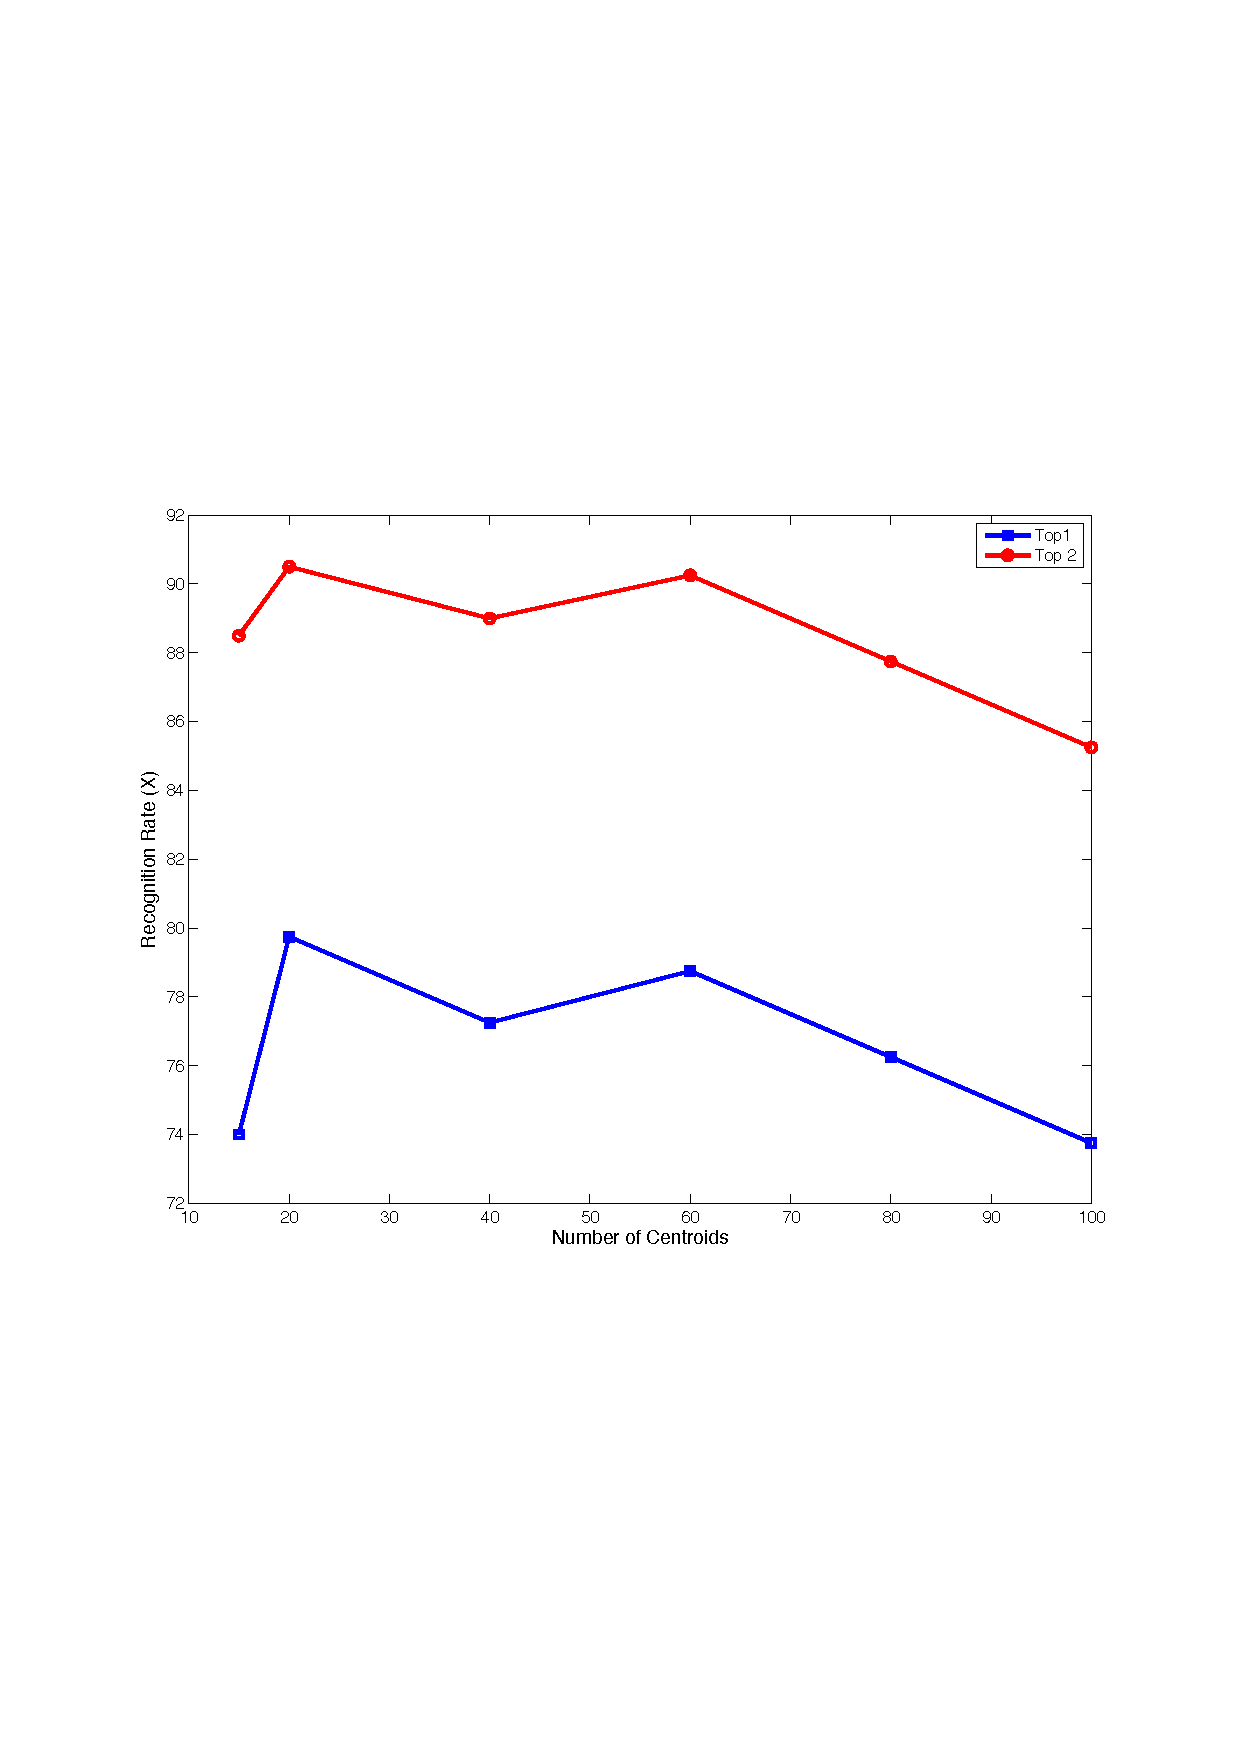
\epsfig{file=vq.pdf, width=12cm}
   \caption{Performance of the concavity feature vector for six different number of centroids}
  \label{vq:fig}
\end{figure}
 
As we can notice, the best results, 79.7\% (Top1) and 90.5\% (Top2), were achieved when using 20 centroids in the vector quantization. After 20 centroids we get no improvement in terms of performance. However, after analysing the confusion matrices for 20 and 60 centroids, we could observe that the classifiers make different mistakes in some classes. The same holds when we compare the confusion matrices produced by the classifiers trained with concavities and global features. This may indicate that combining different configurations of vector quantization and global features could bring some benefits. This will be subject of future investigation. 

Regarding the Chilean database, we have used the best configuration of centroids we found in the experiments with the Brazilian dataset, i.e., 20. Table \ref{top1:tab} shows the confusion matrix for this experiment. Compared with the experiment using global features (Report \#5), the concavity feature set brought an improvement of about 7 percentage points, achieving a recognition rate of 49.1\%, against 42.2\% of the global features. 


\begin{table} [ht!]
\caption {Confusion Matrix for the Chilean dataset using Concavity Features with 20 centroids (\%) - TOP1}
\begin{center}
\begin{tabular}{rrrrrrrrrr} \hline 
 \multicolumn{1}{c}{Class}&
 \multicolumn{1}{c}{1}&
 \multicolumn{1}{c}{2}&
 \multicolumn{1}{c}{3}&
 \multicolumn{1}{c}{4}&
 \multicolumn{1}{c}{5}&
 \multicolumn{1}{c}{6}&
 \multicolumn{1}{c}{7}&
 \multicolumn{1}{c}{8}&
 \multicolumn{1}{c}{9} \\ \hline


1 & \textbf{57.1}&	13.2		&	1.1	&	3.3	&	3.3	&	2.2	&	12.1	&	4.4	&	3.3 \\2 & 9.6			&	\textbf{64.9}&	1.1	&	5.3	&	1.1	&	1.1	&	4.3	&	4.3	&	8.5 \\3 & 20.0		&	25.3		&	\textbf{21.1}	&	0.0	&	10.5	&	8.4	&	3.2	&	10.5	&	1.1\\4 & 16.8		&	11.6		&	2.1	&	\textbf{36.8}	&	9.5	&	4.2	&	6.3	&	9.5	&	3.2\\5 & 24.0		&	16.7		&	17.7	&	2.1	&	\textbf{25.0}	&	2.1	&	8.3	&	3.1	&	1.0\\6 & 17.5		&	4.1			&	1.0	&	1.0	&	4.1	&	\textbf{62.9}	&	8.2	&	1.0	&	0.0\\7 & 10.0		&	3.0			&	0.0	&	4.0	&	1.0	&	14.0	&	\textbf{66.0}	&	0.0	&	2.0\\8 & 10.1		&	16.2		&	6.1	&	5.1	&	3.0	&	2.0	&	5.1	&	\textbf{51.5}	&	1.0\\9 & 5.9			&	0.0			&	0.0	&	0.0	&	0.0	&	0.0	&	0.0	&	5.9	&	\textbf{88.2}\\ \hline

\end{tabular}
\label{top1:tab}
\end{center}
\end{table}


\section{Conclusions}

In this report we have used a vector quantization strategy to convert the real-valued concavity feature vector into a discrete one. Different number of centroids were tried out and the best results were achieved using 20 centroids. For the Brazilian database, the performance of the concavity feature set is slightly inferior to the one achieved by the classifier trained with global features. It is worth of remark, though, that an error analysis may suggest that the combination of these two feature sets may bring some improvements in terms of performance.  

The best configuration found in the experiments using the Brazilian dataset was replicated to the Chilean database. In such a case, the concavity feature set with 20 centroids achieved a recognition rate of 49.1\%, 7 percentage points better than the experiment using global features. Combination of different number of centroids will also be considered in this case to see if  we can further improve these results. It is still worth of remembering that the HMM models should be retrained as soon as we get all the characters available in the Chilean month words. 

 



\bibliographystyle{IEEEbib}
\bibliography{refer}



\end{document}



